\documentclass[../main.tex]
		
		\begin{document}
			\section{Regular Languages}
	\begin{description}
		\item[Task:] Understand when a language is regular and how regular languages are produced. Understand basics of automata theory.
		\item[History:] The term \underline{regular languages} was introduced by Stephen Kleene in 1951. A more descriptive name is \underline{finite-state languages} as we will see that a language is regular $\Leftrightarrow$ it can be recognised by a finite state acceptor, which is a type of finite state machine. \\
		The definition of a regular language is very abstract, though. First, describe what operations the collection of regular languages is closed under: \\
		Let $A$ be a finite set, and let $A^*$ be the set of all words over the alphabet $A$. The regular language over the alphabet $A$ constitutes the smallest collection $C$ of subsets of $A^*$ satisfying that:
		\begin{enumerate}
			\item All finite subsets of $A^*$ belong to $C$.
			\item $C$ is closed under the Kleene star operation (if $M \subseteq A^*$ is inside $C$, \textbf{i.e.} $M \subseteq C$, then $M^* \subseteq C$)
			\item $C$ is closed under concatenation (if $M \subseteq A^*, N \subseteq A^*$ satisfy that $M \subseteq C \land N \subseteq C$, then $M \circ N \subseteq C$)
			\item $C$ is closed under union (if $M \subseteq A^* \land N \subseteq A^*$ satisfy that $M \subseteq C \land N \subseteq C$, then $M \cup N \subseteq C$)
		\end{enumerate}
		\item[Definition:] Let $A$ be a finite set, and let $A^*$ be the set of words over the alphabet $A$. A subset $L$ of $A^*$ is called a \underline{regular language} over the alphabet $A$ if $L = L_m$ for some finite sequence $L_1, L_2,\dots, L_m$ of subsets of $A^*$ with the property that $\forall i, 1 \leq i \leq m, L_i$ satisfies one of the following:
		\begin{enumerate}
			\item $L_i$ is a finite set
			\item $L_i = L_j^*$ for some $j, 1 \leq j \leq i$ (the Kleene star operation applied to one of the previous $L_j's$)
			\item $L_i = L_j \circ L_k$ for some $j, k$ such that $1 \leq j, k < i$ ($L_i$ is a concatenation of previous $L_j$'s)
			\item $L_i = L_j \cup L_k$ for some $j, k$ such that $1 \leq k, j < i$ ($L_i$ is a union of previous $L_j$'s)
		\end{enumerate}
		\item[Example 1:] Let $A = \{0, 1\}$. Let $L = \{0^m 1^n \mid m, n \in \mathbb{N} \hspace{5mm} m \geq 0, n \geq 0 \}$ \\
		$L$ is a regular language. Note that $L$ consists of all strings of first 0's, then 1's or the empty string $\varepsilon$. $0^m1^n$ stands for $m$ 0's followed by $n$ 1's, \textbf{i.e.} $0^m \circ 1^n$. Let us examine $L' = \{0^m \mid m \in \mathbb{N}, m \geq 0 \}$ and $L'' = \{1^n \mid n \in \mathbb{N}, n \geq 0 \}$
		\item[Q:] Can we obtain them via operatons listed among 1 -- 4?
		\item[A:] Yes! Let $M = \{ 0 \} \hspace{10mm} M \subseteq A \subseteq A^*$ and $M^* = L^1 = \{0^m \mid m \in \mathbb{N} \hspace{5mm} m \geq 0 \}$. Let $N = \{1\} \hspace{5mm} N \subseteq A \subseteq A^*$ and $N^* = L'' = \{1^n \mid n \in \mathbb{N}, n \geq 0 \}$. In other words, we can do $L_1 = \{0\}$, $L_2 = \{1\}$, $L_3 = L_1^*$, $l_4 = L_2^*$, $L_5 = L_4 \circ L_5 = L$. Therefore, $L$ is a regular language.
		\item[Example 2] Let $A = \{0, 1\}$. Let $L = \{0^m1^m \mid m \in \mathbb{N}, m \geq 1 \}$. $L$ is the language we used as an example earlier. It turns out $L$ is \underline{NOT} regular. This language consists of strings of 0's followed by an equal number of strings of 1's. For a machine to decide that the string $0^m1^m$ is  inside the language is must store the number of 1's, as it examines the number of 0's or vice versa. The number of strings of the type $0^m1^m$ is not finite, however, so a finite-state machine cannot recognise this language. Heuristically, regular languages correspond to problems that can be solved with finite memory, \textbf{i.e.} we only need to remember one of finitely many things. By contrast, nonregular languages correspond to problems that cannot be solved with finite memory.
		\item[Theorem:] The collection of regular languages $C$ is also closed under the following two operations:
		\begin{enumerate}
			\item Intersection, \textbf{i.e.} if $L', L''$ are regular languages (\textbf{i.e.} $L' \cup L'' \in C$) then their intersection $L' \cap L''$ is a regular language.
			\item Complement, \textbf{i.e.} if $L$ is a regular language (\textbf{i.e.} $L \in C$), then $A* \backslash L$ is a regular language ($A^* \backslash L \in C$).
		\end{enumerate}
		\item[Remark:] These two properties did not come into the definition of a regular language, but they are true and often quite useful.
	\end{description}
	
	\subsection{Finite State Acceptors and Automata Theory}
	\begin{description}
		\item[Definition:] An \underline{automation} is a mathematical model of a computing device. \\
		Plural of automation is \underline{automata}.
		\item[Basic idea:] Reason about computability without having to worry about the complexity of actual implementation. \\
		It is most reasonable to consider at the beginning just finite states automata, \textbf{i.e.} machines with a finite number of internal states. The data entered discretely, and each datum causes the machine to either remain in the same internal state or else make the transition to some other state determined solely by 2 pieces of information:
		\begin{enumerate}
			\item The current state
			\item The input datum
		\end{enumerate}
		In other words, if $S$ is the finite set of all possible states of our finite state machine, then the \underline{transition mapping} $t$ that tells us how the internal state of the machine changes on inputting a datum will depend on the current state $s \in S$ and the imput datum $a$, \textbf{i.e.} the machine will enter a (potentially) new state $s' = t(s, a)$.
		\item[Want] to use finite state machines to recognise languages over some alphabet $A$. Let $L$ be our language.\\
		\begin{table}[h!]
			\centering
			\begin{tabular}{cc}
				\underline{Input} & \underline{Output} \\
				Word $w=a_1\dots a_n, a_i \in A \forall i$ & Yes if $w \in L$ \\
				& No if $w \notin L$
			\end{tabular}
		\end{table}
		Since our finite state machine accepts (\textbf{i.e.} returns \underline{yes} to) $w$ if $w \in L$, we call our machine a \underline{finite state acceptor}. We want to give a rigorous definition of a finite state acceptor. To check $w=a_1 \dots a_n$, we input each $a_i$ starting with $a_1$ and trace how the internal state of the machine changes. $S$ is our set of states of the machine (a finite set). The transition mapping $t$ takes the pair($s, a$) and returns the new state $s'=t(s, a)$ (where $s \in S \land a \in A$) that the machine has reached so $t: S \times A \rightarrow S$. \\
		Some elements and subets of $S$ are important to understand:
		\begin{enumerate}
			\item The initial state $i \in S$ where the machine starts
			\item The subset $F \subseteq S$ of finishing states
		\end{enumerate}
		It turns out that knowing $S, F, i, t, A$ satisfies a finite state acceptor completely.
		\item[Definition:] A finite state acceptor $(S, A, i, t, F)$ consists of a finite set $S$ of states, a finite set $A$ that is the input alphabet, a starting state $i \in S$, a transition mapping $t: S \times A \rightarrow S$, and a set $F$ of finishing states, where $F \subseteq S$.
		\item[Definition:] Let $(S, A, i, t, F)$ be a finite state acceptor, and let $A^*$ denote the set of words over the input alphabet $A$. A word $a_1, a_2\dots a_n$ of length $n$ over the alphabet $A$ is said to be \underline{recognised} or \underline{accepted} by the finite state acceptor if $\exists s_0, s_1, \dots, s_n \in S$ states s.t. $s_0 = i$ (the initial state), $s_n \in F$, and $s_i = t(s_{i-1}, a_i) \forall i \hspace{5mm} 1 \leq i \leq n$.
		\item[Definition:] Let $(S, A, i, t, F)$ be a finite state acceptor. A language $L$ over the alphabet $A$ is said to be \underline{recognised} or \underline{accepted} by the finite state acceptor. \\
		In the definition of a finite state acceptor, $t$ is the transition mapping, which may or may not be a function (hence the careful terminology). This is because finite state acceptors come in 2 flavours:
		\begin{enumerate}
			\item \underline{Deterministic:} every state has exactly one transition for each possible input, \textbf{i.e.} $\forall (s, a) \in S \times A$ $\exists!$ $t(s, a) \in S$. In other words, the transition mapping is a function.
			\item \underline{Non-deterministic:} an input can lead to one, more than one or no transition for a given state. Some $(s, a) \in S \times A$ might be assigned to more than one element of $S$, \textbf{i.e.} the transition mapping is not a function.
		\end{enumerate}
		\item[Surprisingly] $\exists$ algorithm that transforms a non deterministic (thought more complex one) using the powerset construction. \\
		As a result, we have the following theorem:
		\item[Theorem:] A language $L$ over som alphabet $A$ is a regular language $\Leftrightarrow L$ is recognised by a deterministic finite state acceptor with input alphabet $A \Leftrightarrow L$ is recognised by a nondeterministic finite state acceptor with input alphabet $A$.
		\item[Example:] Build a deterministic finite state acceptor for the regular language $L = \{0^m1^n \mid m, n \in \mathbb{N}, m \geq 0, n \geq 0 \}$ \\
		\begin{figure}[h!]
			\centering
			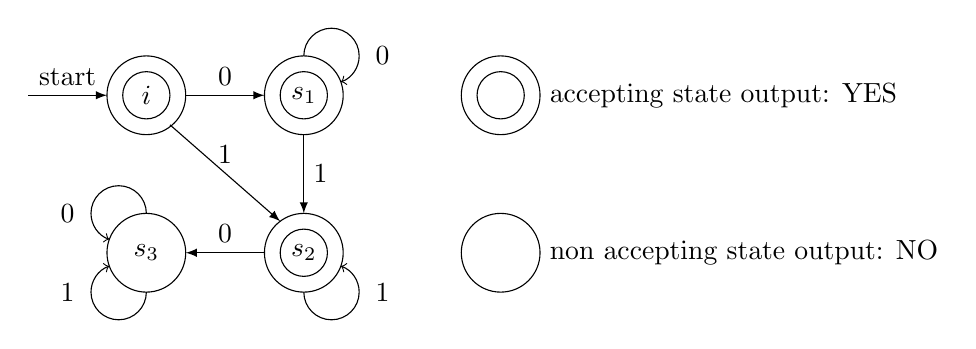
\begin{tikzpicture}
				% Top arrows
				\draw[-latex] (-2, 0)--node[above]{start} (-1, 0);
				\draw[-latex] (0, 0)--node[above]{0} (1, 0);
				% Bottom arrow
				\draw[latex-] (0, -2)--node[above]{0} (1, -2);
				% Middle arrows
				\draw[-latex] (-0.2, -0.375)--node[above]{1} (1.2, -1.6);
				\draw[-latex] (1.5, -0.5)--node[right]{1} (1.5, -1.5);
				
				% Circles
				% Top Left
				\draw (-0.5, 0) circle [radius=0.5];
				\draw (-0.5, 0) circle [radius=0.3] node{$i$};
				
				% Top right
				\draw (1.5, 0) circle [radius=0.5];
				\draw (1.5, 0) circle [radius=0.3] node{$s_1$};
				\draw[->] (1.5, 0.5)  arc(180:-70:10pt);
				\draw (2.5, 0.5) node{0};
				
				% Bottom left
				\draw (-0.5, -2) circle [radius=0.5] node{$s_3$};
				\draw[->](-0.5, -2.5) arc(0:-250:10pt);
				\draw[->](-0.5, -1.5) arc(0:250:10pt);
				\draw (-1.5, -2.5) node{1};
				\draw (-1.5, -1.5) node{0};
				
				% Bottom right
				\draw (1.5, -2) circle [radius=0.5];
				\draw (1.5, -2) circle [radius=0.3] node{$s_2$};
				\draw[->](1.5, -2.5) arc(-180:70:10pt);
				\draw (2.5, -2.5) node{1};
				
				% Legend
				\draw (4, 0) circle [radius=0.5];
				\draw (4, 0) circle [radius=0.3];
				\draw (4.5, 0) node[right]{accepting state output: YES};
				
				\draw (4, -2) circle [radius=0.5];
				\draw (4.5, -2) node[right]{non accepting state output: NO};
			\end{tikzpicture}
		\end{figure}
		~\\
		Accepting states in this examples: $i, s_1, s_2$ \\
		Non accepting states: $s_3$ \\
		Start states: $i$ \\
		Here $S = \{i, s_1, s_2, s_3\} \hspace{5mm} F = \{i, s_1, s_2\} \hspace{5mm} A = \{0, 1\} \hspace{5mm} t: S \times A \rightarrow S \hspace{5mm} t(i, 0) = s_1 \hspace{5mm} t(i, 1) = s_2 \hspace{5mm} t(s_1, 0)  = s_1 \hspace{5mm} t(s_1, 1) = s_2 \hspace{5mm} t(s_2, 0) = s_3 \hspace{5mm} t(s_2, 1) = s_2$ \\
		Let's process some strings:
		\begin{table}[h!]
			\centering
			\begin{tabular}{c|ccc|c|c|c|c|c}
				\cline{1-2} \cline{4-9}
				String & $\varepsilon$ (empty string) & & String & 0 & 0 & 1 & 1 & 1 \\ \cline{1-2} \cline{4-9}
				State (i) & i & & State i & $s_1$ & $s_1$ & $s_2$ & $s_2$ & $s_2$ \\ \cline{1-2} \cline{4-9}
				Output & YES & & Output & \multicolumn{5}{c}{YES} \\ \cline{1-2} \cline{4-9}
			\end{tabular}
		\end{table}
		\begin{table}[h!]
			\centering
			\begin{tabular}{c|c|ccc|ccc|c|c|c|c}
				\cline{1-3} \cline{5-6} \cline{8-12}
				String & 1 & 1 & & String & 1 & & String & 0 & 1 & 0 & 1 \\ \cline{1-3} \cline{5-6} \cline{8-12}
				State i & $s_2$ & $s_2$ & & State i & $s_2$ & & State i & $s_1$ & $s_2$ & $s_3$ & $s_3$ \\ \cline{1-3} \cline{5-6} \cline{8-12}
				Output & \multicolumn{2}{c}{YES} & & Output & YES & & Output & \multicolumn{4}{c}{NO} \\ \cline{1-3} \cline{5-6} \cline{8-12}
			\end{tabular}
		\end{table}
		~\\
		Now that we really understand what a finite state acceptor is, we can develop a criterion for recognised regular languages called the \underline{Myhill-Nerode theorem} based on an equivalence relation we can set up on words in our language over the alphabet $A$.
		\item[Definition:] Let $x, y \in L$, a language over the alphabet $A$. We call $x$ and $y$ equivalent over $L$ denoted by $x \equiv_L y$ if $\forall w \in A^*, xw \in L \Leftrightarrow yw \in L$.
		\item[Note:] $xw$ means the concatenation $x \circ w$, and $yw$ is the concatenation $y \circ w$.
		\item[Idea:] If $x \equiv_L y$, then $x$ and $y$ place our finite state acceptor into the \underline{same state} $s$.
		\item[Notation:] Let $L/N$ be the set of equivalence classes determined by the equivalence relation $\equiv_L$.
		\item[The Myhill-Nerode Theorem:] Let $L$ be a language over the alphabet $A$. If the set $L/N$ of equivalence classes in $L$ is infinite, then $L$ is not a regular language.
		\item[Sketch of Proof:] All element of one equivalence class in $L/N$ place our automation into the same state $s$. Elements of distinct equivalence classes place the automation into distinct state, \textbf{i.e.} if $[x], [y] \in L/N$ and $[x] \neq [y]$, then all elements of $[x]$ place the automation into some state $s$, while all elements of $[y]$ place the automation into some state $s'$, with $s \neq s' \Rightarrow$ an automation that can recognise $L$ has \underline{as many} states at the number of equivalence classes in $L/N$, but $L/N$ is \underline{NOT} finite $\Rightarrow L$ cannot be recognised by a finite state automation $\Rightarrow L$ is not regular by the theorem above.
		\item[qed]
	\end{description}
	

\end{document}